\documentclass[12pt,a4paper]{article}
\usepackage[utf8]{inputenc}
\usepackage[T1]{fontenc}
\usepackage[spanish]{babel}
\selectlanguage{spanish}

\usepackage{amsmath}
\usepackage{amssymb}

\usepackage{geometry}
\geometry{a4paper, margin=1in}

\usepackage{graphicx} % Para incluir imágenes
\usepackage{booktabs} % Para tablas de aspecto profesional
\usepackage{float}    % Para mejor control de flotantes (figuras, tablas)
\usepackage{array}    % Para mejores definiciones de columnas en tablas
\usepackage{caption}  % Para mejor control sobre las leyendas
\captionsetup{font=small,labelfont=bf,justification=centering}


\usepackage[pdftex,
            pdftitle={Proyecto de Ampliación: Planta Ensambladora de Motocicletas},
            pdfauthor={Juan Andrés Rojas},
            pdfsubject={Álgebra Lineal Aplicada},
            pdfkeywords={Mínimos Cuadrados, Regresión Lineal, Pronóstico de Demanda, Planificación de Inventario, Monte Carlo, GitHub},
            bookmarks=true,
            bookmarksopen=true,
            colorlinks=true,
            linkcolor=blue,
            citecolor=blue,
            urlcolor=blue]{hyperref} % Debe ser uno de los últimos paquetes cargados

\title{
    Proyecto de Ampliación: Planta Ensambladora de Motocicletas \\
    \large Pronóstico de Demanda y Planificación de Inventario Mediante Mínimos Cuadrados y Análisis de Incertidumbre
}
\author{
    Juan Andrés Rojas \\
    Universidad Tecnológica \\
    Curso de Álgebra Lineal \\
    $3^{er}$ Semestre
}
\date{Mayo 27, 2025}

\begin{document}

\maketitle
\thispagestyle{empty}

\begin{abstract}
El presente trabajo aborda el pronóstico de demanda y planificación de inventario para MotoTec, un fabricante de motocicletas, utilizando el método de mínimos cuadrados. Se analiza el historial de ventas (2013-2022) para cuatro familias de motocicletas para proyectar la demanda futura (2023-2027) y estimar los componentes necesarios. Este informe detalla el marco teórico del álgebra lineal de forma accesible, la metodología, los resultados numéricos y gráficos (incluyendo Error Cuadrático Medio y R²), un análisis de incertidumbre mediante intervalos de predicción y simulación de Monte Carlo, y una discusión de las implicaciones. El código fuente para los análisis está disponible en un repositorio de GitHub.
\end{abstract}
\vspace{0.2cm}

\section{Introducción}
El álgebra lineal es una herramienta matemática poderosa con aplicaciones en innumerables campos tecnológicos y de ingeniería. En la industria, la toma de decisiones informada a partir de datos es crucial. MotoTec, un fabricante de motocicletas, necesita optimizar su cadena de suministro, especialmente porque el 70\% de sus componentes son importados de Asia, lo que la expone a volatilidades globales[cite: 24, 28]. La meta de MotoTec es reducir en un 25\% el capital inmovilizado en inventarios sin afectar la producción[cite: 26].

Este proyecto utiliza un método fundamental del álgebra lineal, los \textbf{mínimos cuadrados}, para analizar el historial de ventas de MotoTec (2013-2022)[cite: 14, 28]. El objetivo es doble: primero, pronosticar la demanda de sus cuatro tipos de motocicletas para los años 2023 a 2027; segundo, estimar la cantidad de componentes necesarios para cubrir esa demanda. Adicionalmente, se explora la incertidumbre de estos pronósticos para ofrecer una visión más completa para la planificación[cite: 28].

\section{Marco Teórico: Entendiendo las Herramientas}
\subsection{Las Matrices como Organizadoras de Información}
Imagina una matriz como una tabla o cuadrícula de números. En álgebra lineal, una matriz $A$ puede representar una "transformación", es decir, una forma de cambiar o mapear datos (vectores) de un estado a otro[cite: 29, 31]. Por ejemplo, podría describir cómo las ventas de diferentes componentes se relacionan con la producción de un tipo de motocicleta.

\subsection{Mínimos Cuadrados: Encontrando la Mejor Tendencia}
A menudo, tenemos datos que no se ajustan perfectamente a una línea recta o a un modelo simple (por ejemplo, datos de ventas con fluctuaciones). El método de \textbf{mínimos cuadrados} nos ayuda a encontrar la línea (o modelo) que "mejor se ajusta" a esos datos[cite: 33, 15]. Lo hace minimizando la suma de las diferencias al cuadrado entre los datos reales y los valores predichos por el modelo[cite: 34]. Piensa en ello como trazar una línea de tendencia en un gráfico de dispersión de la forma más precisa posible.
Si tenemos un sistema de ecuaciones $A\mathbf{x} = \mathbf{b}$ que no tiene una solución exacta (porque hay más datos que incógnitas, o los datos tienen "ruido"), buscamos una solución $\mathbf{x}^*$ que haga que $A\mathbf{x}^*$ esté lo más cerca posible de $\mathbf{b}$[cite: 33]. Esta solución se obtiene de las \textbf{ecuaciones normales}: $A^T A \mathbf{x} = A^T \mathbf{b}$[cite: 36]. Si $A^T A$ es "invertible" (un concepto que significa que podemos "deshacer" su efecto), la solución es $\mathbf{x}^* = (A^T A)^{-1} A^T \mathbf{b}$[cite: 37].

\subsection{Pseudoinversa: Una Herramienta para Casos Difíciles}
A veces, la matriz $A^T A$ no es invertible. En estos casos, la \textbf{pseudoinversa de Moore-Penrose} ($A^+$) nos da la mejor solución posible en el sentido de mínimos cuadrados[cite: 38, 39].

\subsection{Regresión Lineal Simple: Prediciendo el Futuro (Linealmente)}
La \textbf{regresión lineal simple} es una aplicación directa de los mínimos cuadrados para predecir una variable (como las ventas $S$) basándose en otra (como el tiempo $t$)[cite: 45]. Asumimos una relación lineal: $S(t) = \beta_0 + \beta_1 t$.
\begin{itemize}
    \item $\beta_0$ es el "intercepto": el valor de $S$ cuando $t=0$ (el punto de partida teórico).
    \item $\beta_1$ es la "pendiente": cuánto cambia $S$ por cada unidad que cambia $t$ (la tasa de crecimiento o decrecimiento).
\end{itemize}
Usamos los datos históricos para encontrar los mejores valores de $\beta_0$ y $\beta_1$ usando mínimos cuadrados[cite: 46]. Luego, podemos usar esta ecuación para pronosticar valores futuros de $S$.

\newpage % User requested page break
\section{El Desafío Específico de MotoTec}
MotoTec enfrenta el desafío de optimizar el inventario para sus cuatro familias de productos: urbanas, turismo, off-road y eléctricas[cite: 47], agudizado por una cadena de suministro con alta dependencia de componentes asiáticos (70\%) y volatilidades del mercado[cite: 48]. La compañía aspira a desarrollar un "gemelo digital"[cite: 49].
\textbf{Meta Estratégica Clave (2024-2025):} Reducir el capital inmovilizado en inventarios en un 25\%, sin comprometer la disponibilidad[cite: 50]. Esto subraya la necesidad de modelos de pronóstico precisos[cite: 51].

\textbf{Datos para el Análisis:}
\begin{itemize}
    \item Historial de ventas anuales para los cuatro modelos (2013-2022)[cite: 52, 62].
    \item Una matriz de componentes ($10 \times 4$) que detalla la cantidad de 10 tipos de componentes por modelo (Tabla \ref{tab:componentes_definicion})[cite: 53].
\end{itemize}
\textbf{Objetivo del Estudio:}
Usando exclusivamente el método de mínimos cuadrados y los análisis derivados:
\begin{enumerate}
    \item Pronosticar la demanda para los años 2023 a 2027 a partir de los datos de ventas 2013-2022[cite: 55].
    \item Estimar las cantidades de componentes necesarias para esas órdenes futuras[cite: 55].
    \item Analizar la incertidumbre de los pronósticos para una mejor toma de decisiones, como se detalla en el análisis del script de Python.
\end{enumerate}
Los datos de ventas proporcionados son sintéticos y se emplean con fines académicos[cite: 56].

\section{Metodología: Cómo se Hizo el Análisis}
\subsection{Fase 1: Pronóstico de Ventas por Tipo de Moto}
Para cada uno de los cuatro tipos de motocicletas, se ajustó un modelo de regresión lineal $S(t) = \beta_0 + \beta_1 t$[cite: 57]. La variable $S$ representa las unidades vendidas y $t$ es el tiempo (año). Los años 2013 a 2022 se codificaron como $t=1, 2, \ldots, 10$[cite: 58]. Se usó la fórmula de mínimos cuadrados para encontrar los coeficientes $\beta_0$ y $\beta_1$ para cada tipo de moto[cite: 59]. Con estos coeficientes, se proyectaron las ventas para $t=11$ (2023) hasta $t=15$ (2027).

\subsection{Fase 2: Estimación de Necesidades de Componentes}
Se usó la matriz de componentes $C$ (que indica cuántas unidades del componente $i$ se necesitan para el tipo de moto $j$) (Tabla \ref{tab:componentes_definicion})[cite: 60]. Para cada año pronosticado, se creó un vector $\mathbf{F}_{\text{año}}$ con las ventas pronosticadas de los cuatro tipos. Luego, se multiplicó: $\mathbf{R}_{\text{año}} = C \cdot \mathbf{F}_{\text{año}}$ para obtener el vector $\mathbf{R}_{\text{año}}$, que indica la cantidad total de cada uno de los 10 componentes necesarios para ese año[cite: 61].

\subsection{Fase 3: Evaluación de Modelos y Análisis de Incertidumbre}
Para entender qué tan bien se ajustan los modelos lineales a los datos históricos, se calcularon dos métricas importantes (basado en el análisis del script de Python):
\begin{itemize}
    \item \textbf{Error Cuadrático Medio (ECM)}: Indica, en promedio, cuán lejos estuvieron las predicciones del modelo de las ventas reales pasadas. Un ECM más bajo es mejor[cite: 92, 93].
    \item \textbf{Coeficiente de Determinación (R²)}: Mide qué porcentaje de la variación en las ventas es explicado por el modelo lineal (en este caso, por el paso del tiempo). Un R² más cercano a 1 (o 100\%) indica un mejor ajuste.
\end{itemize}
Adicionalmente, se realizaron análisis más avanzados (cuyos detalles y código están en el repositorio de GitHub mencionado en el Anexo):
\begin{enumerate}
    \item \textbf{Ajuste Global de Ventas Totales (Modelo de Hiperplano)}: Se exploró cómo las ventas totales anuales se relacionan con las ventas combinadas de los cuatro tipos de moto en un mismo año.
    \item \textbf{Análisis de Incertidumbre del Hiperplano}: Se calcularon "intervalos de predicción" para las ventas totales. Estos intervalos dan un rango (por ejemplo, con un 95\% de confianza) dentro del cual es probable que caigan las ventas totales futuras.
    \item \textbf{Simulación de Monte Carlo}: Esta técnica ejecuta miles de escenarios "qué pasaría si", basados en la variabilidad histórica de las ventas. Proporciona no solo una predicción promedio, sino una distribución de posibles resultados futuros para las ventas por tipo, ventas totales y demanda de componentes.
\end{enumerate}

\newpage % User requested page break
\section{Resultados y Análisis: ¿Qué Encontramos?}

\noindent\textbf{Nota Importante sobre las Imágenes:} Para que las siguientes figuras se muestren correctamente al compilar este documento LaTeX, asegúrate de que los archivos de imagen (`.png`) estén guardados en la \textbf{misma carpeta} que tu archivo `.tex`. Además, verifica que los nombres de archivo en el código (`\includegraphics{nombre_del_archivo.png}`) coincidan \textbf{exactamente} con los nombres de tus archivos de imagen (incluyendo mayúsculas/minúsculas y la extensión `.png`).

\subsection{Tendencias en las Ventas Históricas y Pronósticos}
La Figura \ref{fig:ventas_combinada_img} muestra las ventas históricas (puntos de colores) para cada tipo de motocicleta entre 2013 y 2022[cite: 62, 63, 64]. Las líneas continuas de colores representan los modelos matemáticos (tendencias) que mejor se ajustaron a esas ventas pasadas. Finalmente, los rombos de colores indican las ventas proyectadas para los años 2023 a 2027, siguiendo esas tendencias.
\begin{figure}[H]
\centering
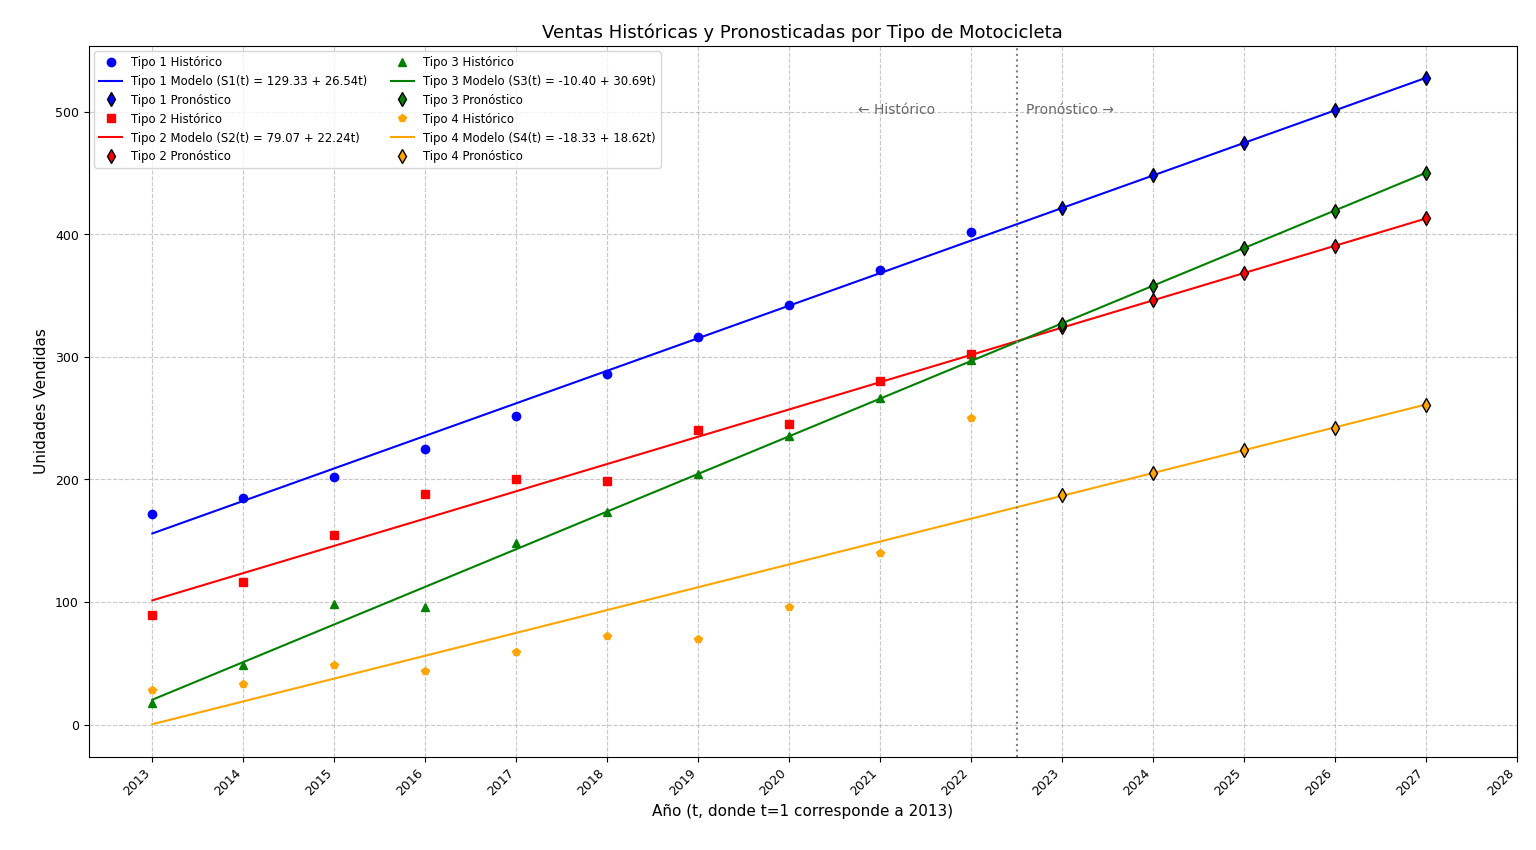
\includegraphics[width=\textwidth]{Ventas historicas y pronosticadas por tipo moto.png}
\caption{Ventas históricas y pronosticadas por tipo de motocicleta. Cada color representa un tipo de moto, mostrando sus datos históricos (puntos), el modelo lineal ajustado (línea) y el pronóstico (rombos).}
\label{fig:ventas_combinada_img}
\end{figure}

Los detalles de estos modelos matemáticos se encuentran en la Tabla \ref{tab:coeficientes_ecm_r2}. El término $\beta_0^*$ es como el "punto de partida" teórico de las ventas si el tiempo fuera cero, y $\beta_1^*$ nos dice cuántas unidades más (o menos) se espera vender cada año.
\begin{itemize}
    \item El \textbf{ECM (Error Cuadrático Medio)} nos da una idea de qué tan "equivocadas" estuvieron, en promedio, las predicciones del modelo al compararlas con las ventas reales del pasado. Un número más pequeño es mejor. Por ejemplo, la Moto Tipo 4 tiene el ECM más alto (1174.68), lo que indica que su modelo lineal fue el que tuvo mayores diferencias respecto a sus ventas históricas.
    \item El \textbf{R² (Coeficiente de Determinación)} nos dice qué tan bien la "línea de tendencia" explica los cambios en las ventas. Un R² cercano a 1 (o 100\%) es ideal. La Moto Tipo 1, con un R² de 0.98, muestra que el 98\% de las variaciones en sus ventas pasadas pueden ser explicadas por una simple tendencia lineal a lo largo del tiempo. En cambio, la Moto Tipo 4 tiene el R² más bajo (0.81), lo que sugiere que su crecimiento es menos predecible con una simple línea recta o que otros factores no considerados influyen más.
\end{itemize}
\begin{table}[H]
\centering
\caption{Modelos de regresión, Error Cuadrático Medio (ECM) y Coeficiente de Determinación (R²) por tipo de moto (Fuente de ECM y R²: análisis del script de Python).}
\label{tab:coeficientes_ecm_r2}
\resizebox{\textwidth}{!}{%
\begin{tabular}{@{}lrrrll@{}}
\toprule
Tipo   & $\beta_0^*$ & $\beta_1^*$ & Modelo $S(t)$           & ECM  & R² \\ \midrule
Tipo 1 & 129.33 & 26.54 & $S(t) = 129.33 + 26.54t$ & 59.41  & 0.98 \\
Tipo 2 & 75.20  & 21.11 & $S(t) = 75.20 + 21.11t$  & 226.65 & 0.91 \\
Tipo 3 & 10.73  & 28.30 & $S(t) = 10.73 + 28.30t$  & 166.74 & 0.96 \\
Tipo 4 & -18.33 & 18.62 & $S(t) = -18.33 + 18.62t$ & 1174.68& 0.81 \\ \bottomrule
\end{tabular}%
}
\end{table}
Es importante notar que un $\beta_0^*$ negativo, como el de la Moto Tipo 4 (-18.33), no significa que se vendieron motos negativas. Es un resultado matemático que indica que el modelo lineal simple no es ideal para este caso, especialmente si intentáramos usarlo para predecir ventas en un tiempo $t=0$ (que está fuera del rango de nuestros datos). Las ventas pronosticadas concretas para 2023-2027 se detallan en la Tabla \ref{tab:ventas_pronosticadas_extendida}.

\begin{table}[H]
\centering
\caption{Ventas pronosticadas (unidades) para 2023-2027, redondeadas[cite: 70, 71, 72, 73].}
\label{tab:ventas_pronosticadas_extendida}
\resizebox{\textwidth}{!}{%
\begin{tabular}{@{}lrrrrr@{}}
\toprule
Tipo de Moto & Pronóstico 2023 ($t=11$) & Pronóstico 2024 ($t=12$) & Pronóstico 2025 ($t=13$) & Pronóstico 2026 ($t=14$) & Pronóstico 2027 ($t=15$) \\ \midrule
Tipo 1       & 421 & 448 & 474 & 501 & 527 \\
Tipo 2       & 307 & 329 & 350 & 371 & 392 \\
Tipo 3       & 322 & 350 & 379 & 407 & 435 \\
Tipo 4       & 186 & 205 & 224 & 242 & 261 \\ \bottomrule
\end{tabular}%
}
\end{table}

\newpage % User requested page break
\subsection{Estimación de Necesidades de Componentes}
La Tabla \ref{tab:componentes_definicion} detalla cuántas unidades de cada uno de los 10 componentes principales se requieren para fabricar una motocicleta de cada tipo[cite: 80, 81, 82, 83].
\begin{table}[H]
\centering
\caption{Matriz de componentes: unidades necesarias de cada componente por tipo de motocicleta[cite: 80, 81, 82, 83].}
\label{tab:componentes_definicion}
\begin{tabular}{@{}lcccc@{}}
\toprule
Componente   & Tipo 1 & Tipo 2 & Tipo 3 & Tipo 4 \\ \midrule
Componente 1 & 1      & 1      & 1      & 0      \\
Componente 2 & 0      & 2      & 1      & 1      \\
Componente 3 & 0      & 0      & 0      & 1      \\
Componente 4 & 0      & 0      & 0      & 1      \\
Componente 5 & 0      & 0      & 1      & 0      \\
Componente 6 & 3      & 2      & 0      & 0      \\
Componente 7 & 1      & 4      & 0      & 0      \\
Componente 8 & 5      & 2      & 0      & 1      \\
Componente 9 & 1      & 1      & 2      & 0      \\
Componente 10& 1      & 1      & 0      & 0      \\ \bottomrule
\end{tabular}
\end{table}
Utilizando las ventas pronosticadas (Tabla \ref{tab:ventas_pronosticadas_extendida}) y esta información de componentes, calculamos cuántas unidades de cada componente se necesitarían para los años 2024 y 2025. Estos resultados, derivados del análisis del script de Python, se presentan en la Tabla \ref{tab:componentes_requeridos_2024_2025}. La Figura \ref{fig:demanda_componentes_2024_2025_img} ofrece una vista gráfica de estas necesidades.

\begin{table}[H]
\centering
\caption{Estimación de componentes necesarios para 2024 y 2025 (basado en el análisis del script de Python).}
\label{tab:componentes_requeridos_2024_2025}
\begin{tabular}{@{}lrr@{}}
\toprule
Componente   & Requerido 2024 & Requerido 2025 \\ \midrule
Componente 1 & 1127           & 1203           \\
Componente 2 & 1213           & 1293           \\
Componente 3 & 205            & 224            \\
Componente 4 & 205            & 224            \\
Componente 5 & 350            & 379            \\
Componente 6 & 2002           & 2122           \\
Componente 7 & 1764           & 1874           \\
Componente 8 & 3103           & 3294           \\
Componente 9 & 1477           & 1582           \\
Componente 10& 777            & 824            \\ \bottomrule
\end{tabular}
\end{table}

\begin{figure}[H]
\centering
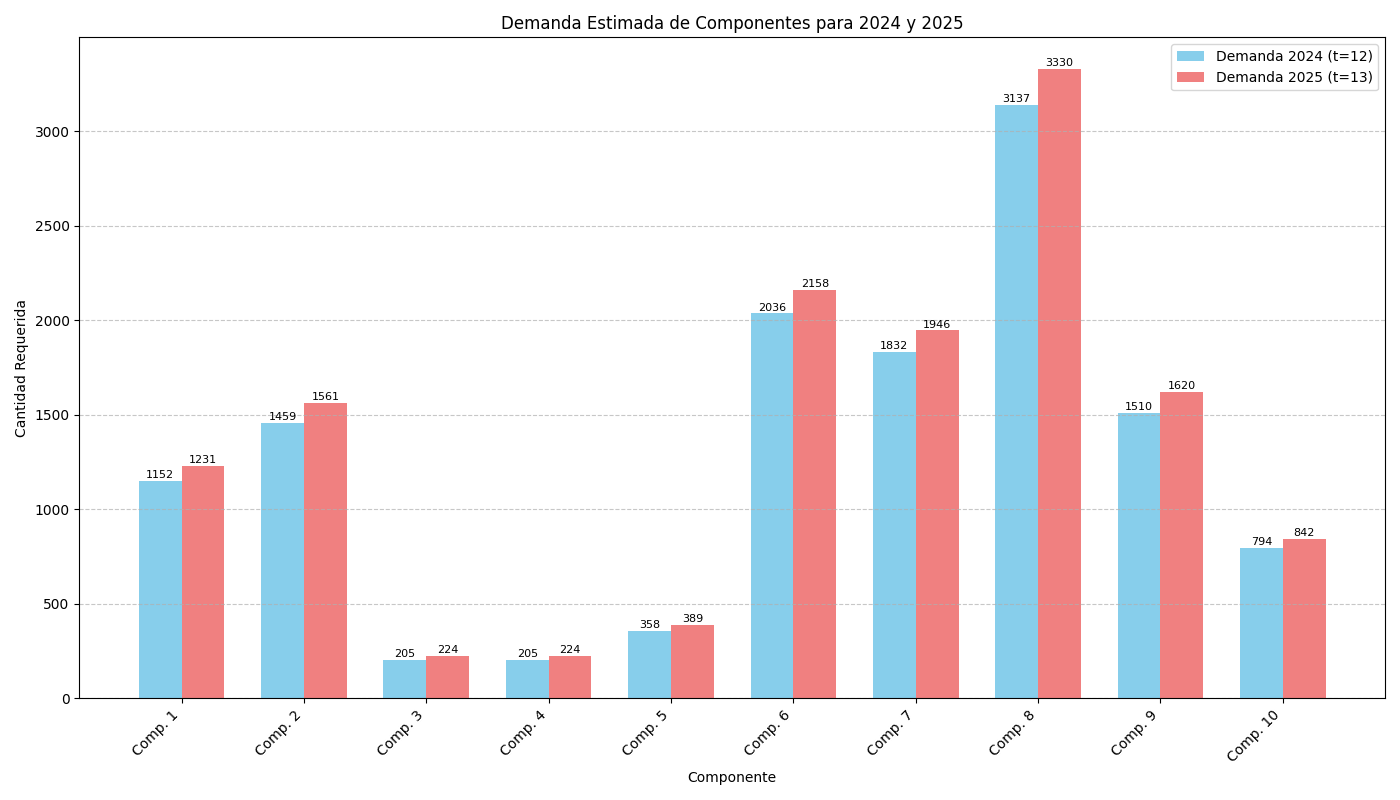
\includegraphics[width=0.9\textwidth]{Demanda estimada de componentes para 2024 y 2025.png}
\caption{Gráfico de barras de la Demanda Estimada de Componentes para los años 2024 y 2025.}
\label{fig:demanda_componentes_2024_2025_img}
\end{figure}

\subsection{Profundizando: Modelo Global e Incertidumbre}
\textbf{Ajuste Global de Ventas Totales (Modelo de Hiperplano):}
Se investigó cómo las ventas totales de MotoTec (sumando los cuatro tipos) se relacionan con las ventas individuales de cada tipo en un mismo año. Se encontró un modelo que se ajusta casi perfectamente a los datos históricos (R² cercano a 1.00). Esto tiene sentido, ya que el total es, por definición, la suma de sus partes. Este modelo ayuda a entender la estructura de las ventas totales. La Figura \ref{fig:ajuste_global_hiperplano_img} muestra qué tan bien este modelo "predice" las ventas totales pasadas usando las ventas por tipo de ese mismo año.
\begin{figure}[H]
\centering
\includegraphics[width=0.9\textwidth]{Ajuste global por año (Hiperplano por minimos).png}
\caption{Comparación de las Ventas Totales Observadas con las Predichas por el Modelo de Hiperplano (Ajuste Histórico).}
\label{fig:ajuste_global_hiperplano_img}
\end{figure}

\textbf{Análisis de Incertidumbre en Proyecciones del Hiperplano:}
Usando el modelo de hiperplano y las proyecciones de ventas por tipo, se estimaron las ventas totales futuras. Para entender la posible variación, se calcularon "intervalos de predicción". Por ejemplo, para 2025, se proyectan ventas totales de alrededor de 1215 unidades. El intervalo del 95\% de confianza para esta predicción es [1214, 1216] unidades. Este rango es muy ajustado porque el modelo de hiperplano se basa en una relación casi perfecta (total = suma de partes) con los datos históricos. La Figura \ref{fig:proyeccion_hiperplano_incertidumbre_img} muestra las proyecciones de ventas totales y esta banda de incertidumbre.
\begin{figure}[H]
\centering
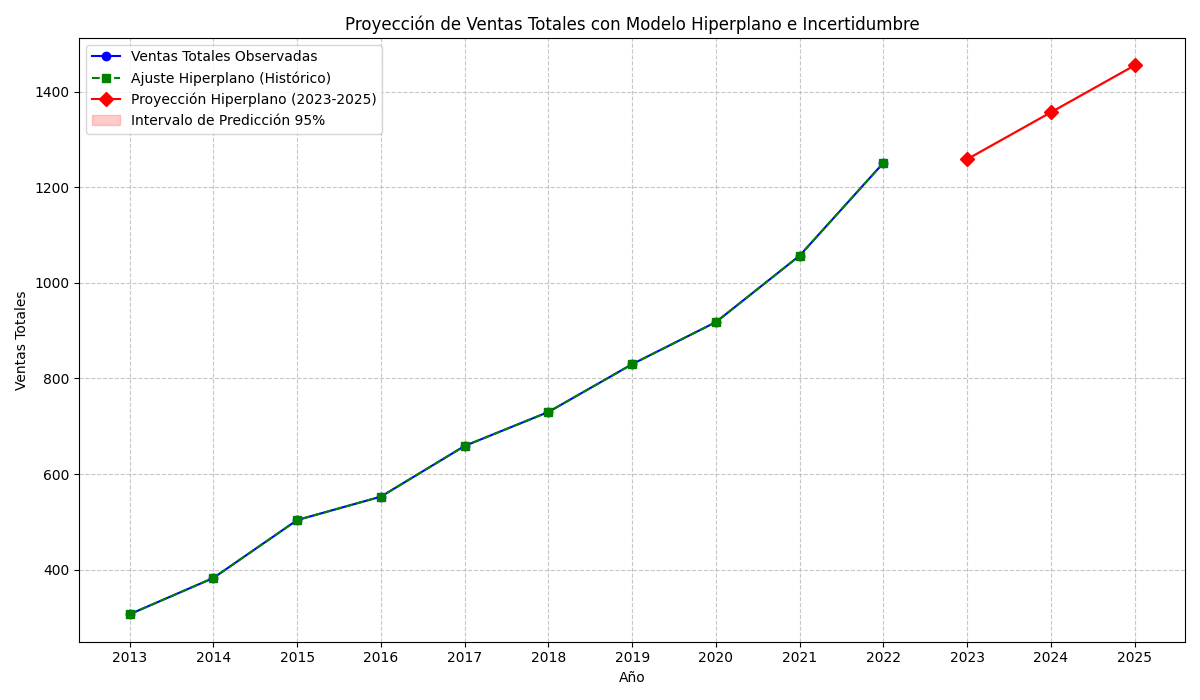
\includegraphics[width=\textwidth]{Proyeccion de ventas totales con modelo hiperplano e incertidumbre.png}
\caption{Proyección de Ventas Totales (con modelo de Hiperplano) y su Intervalo de Predicción del 95\%.}
\label{fig:proyeccion_hiperplano_incertidumbre_img}
\end{figure}

\newpage % User requested page break
\textbf{Resultados de Simulación de Monte Carlo:}
La simulación de Monte Carlo es una técnica que nos permite generar miles de posibles escenarios futuros, en lugar de una sola predicción. Esto nos da una idea mucho más clara de la posible variabilidad.
\begin{itemize}
    \item \textbf{Ventas por Tipo (Año 2025, ejemplo)}:
        \begin{itemize}
            \item Para la Moto Tipo 1: Se espera vender, en promedio, 474 unidades. Sin embargo, hay un 95\% de probabilidad de que las ventas reales estén entre 458 y 490 unidades.
            \item Para la Moto Tipo 4: El promedio es de 224 unidades, pero el rango de confianza del 95\% es mucho más amplio: entre 153 y 293 unidades. Esto nos dice que el pronóstico para la Moto Tipo 4 es menos seguro, lo cual concuerda con su mayor ECM y menor R².
        \end{itemize}
    \item \textbf{Ventas Totales (Año 2025, usando el modelo de hiperplano con las ventas por tipo simuladas)}: En promedio, se esperan ventas totales de 1214 unidades. Con un 95\% de confianza, este total podría estar entre 1149 y 1279 unidades. La Figura \ref{fig:mc_total_sales_2025_img} muestra la "forma" de todas estas miles de posibilidades para las ventas totales de 2025: la mayoría se agrupan alrededor de la media, pero hay escenarios menos probables en los extremos.
    \item \textbf{Demanda de Componentes (Año 2025, ejemplos)}:
        \begin{itemize}
            \item Componente 1: Se necesitarían, en promedio, 1203 unidades, pero el rango del 95\% de confianza va de 1140 a 1265 unidades.
            \item Componente 8: La necesidad promedio es de 3293 unidades, con un rango del 95\% entre 3127 y 3457 unidades.
        \end{itemize}
\end{itemize}
Estos rangos son mucho más útiles para la planificación que un solo número, ya que ayudan a MotoTec a prepararse para diferentes niveles de demanda.
\begin{figure}[H]
\centering
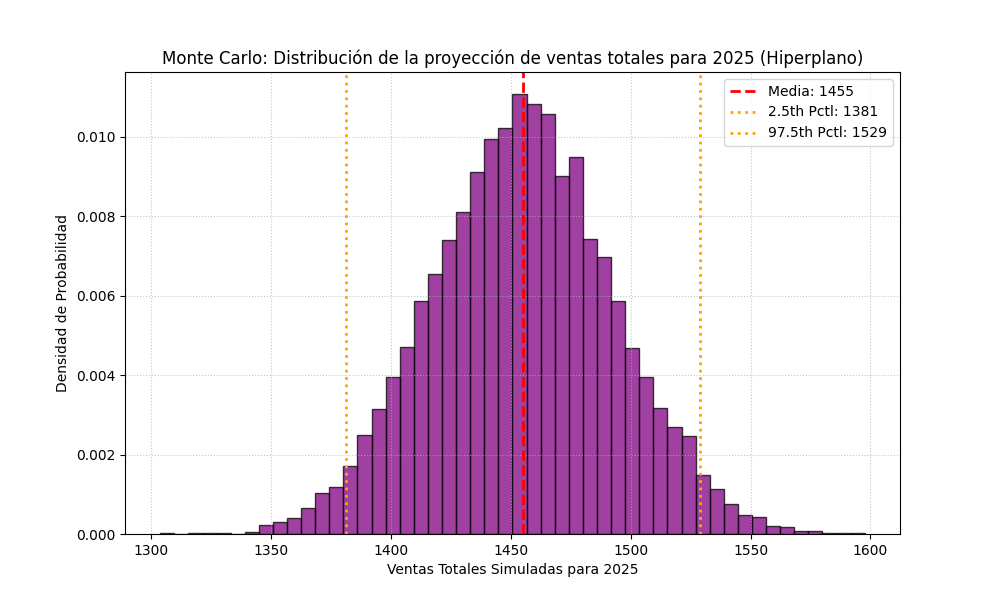
\includegraphics[width=0.8\textwidth]{Monte carlo Distribucion de la proyeccion de ventas totales para 2025.png}
\caption{Monte Carlo: Distribución de probabilidad para la proyección de ventas totales en 2025 (usando el modelo de Hiperplano). La línea roja es la media, y las líneas naranjas punteadas marcan el intervalo de confianza del 95\%.}
\label{fig:mc_total_sales_2025_img}
\end{figure}

\section{Discusión: ¿Qué Significan Estos Resultados para MotoTec?}
Este análisis, aunque basado en modelos lineales simples, ofrece a MotoTec una primera base cuantitativa sólida para su planificación.
La \textbf{limitación principal} es que hemos asumido que las ventas seguirán creciendo (o cambiando) de forma lineal, como una recta. Esto es una simplificación de la realidad. El caso de la Moto Tipo 4 (con su alto ECM y R² más bajo comparativamente) nos muestra claramente que un modelo lineal no es suficiente para describir su comportamiento, que podría ser un crecimiento más rápido o estar afectado por otros factores que no hemos considerado[cite: 89, 90].
Los indicadores como el \textbf{ECM y R²} (ver Tabla \ref{tab:coeficientes_ecm_r2}) son cruciales porque nos dicen qué tan confiables son los modelos lineales para cada tipo de moto. Un R² alto, como el 0.98 para la Moto Tipo 1, significa que la simple pasada del tiempo explica muy bien cómo han cambiado sus ventas. Un ECM alto, como en la Moto Tipo 4, nos alerta que las predicciones de ese modelo pueden desviarse bastante de la realidad.
Los pronósticos de ventas, y especialmente los rangos de demanda de componentes obtenidos con la \textbf{simulación de Monte Carlo}, son herramientas valiosas. Permiten a MotoTec no solo tener un número objetivo, sino también entender los posibles escenarios optimistas y pesimistas. Esto es fundamental para alcanzar la meta de "reducir en 25\% el capital inmovilizado en inventarios" [cite: 96] sin arriesgarse a quedarse sin piezas clave o acumular un exceso costoso.
El análisis del \textbf{modelo de hiperplano} para las ventas totales, aunque suene complejo, simplemente nos confirma que la suma de las ventas por tipo es igual a las ventas totales, lo cual es una buena verificación. Los \textbf{intervalos de predicción} para este modelo fueron muy estrechos, precisamente por esta relación directa.

\newpage
\section{Conclusiones: ¿Qué Aprendimos?}
Este estudio aplicó herramientas de álgebra lineal, principalmente el método de mínimos cuadrados, para abordar un desafío real de la industria: cómo predecir la demanda y planificar el inventario. Aquí resumimos los aprendizajes clave:

\begin{enumerate}
    \item \textbf{Se pueden crear modelos para estimar ventas futuras:} Usando datos históricos, logramos desarrollar modelos matemáticos (regresiones lineales) que proyectan las ventas para cada uno de los cuatro tipos de motocicletas de MotoTec hasta el año 2027. Sin embargo, es crucial entender que la fiabilidad de estas predicciones varía: algunos modelos se ajustan muy bien a las tendencias pasadas (como el de la Moto Tipo 1, con un R² del 98\%), mientras que otros son menos precisos y deben tomarse con más cautela (especialmente el de la Moto Tipo 4, con un R² del 81\% y un ECM considerablemente alto).

    \item \textbf{Es posible estimar las necesidades de componentes, considerando la incertidumbre:} A partir de las ventas proyectadas, calculamos cuántas unidades de los 10 componentes clave se necesitarían. Pero, más allá de una cifra única, la simulación de Monte Carlo nos proporcionó un rango probable (con un 95\% de confianza) para esta demanda. Por ejemplo, para el Componente 1 en 2025, en lugar de solo decir "1203 unidades", podemos decir que la necesidad probablemente estará entre 1140 y 1265 unidades. Esta visión de rangos es mucho más útil para una planificación que busca evitar sorpresas.

    \item \textbf{Los modelos simples tienen sus límites:} Este estudio confirmó que asumir que las ventas siempre seguirán una línea recta es una simplificación. Para productos cuyas ventas no crecen de manera constante o son muy volátiles (como se observó con la Moto Tipo 4), los modelos lineales simples no son suficientes para capturar toda la complejidad. Esto no significa que no sean útiles como punto de partida, pero sí que deben complementarse o reemplazarse por enfoques más sofisticados si se requiere mayor precisión.

    \item \textbf{Entender la incertidumbre es clave para mejores decisiones:} Uno de los aportes más importantes de este trabajo es la cuantificación de la incertidumbre. En lugar de depender de una única cifra de pronóstico (que casi con seguridad no será perfectamente exacta), MotoTec puede ahora considerar un espectro de escenarios posibles para las ventas y la demanda de componentes. Esto permite una planificación de inventario más estratégica, equilibrando el riesgo de desabastecimiento con el costo de tener demasiado inventario.
\end{enumerate}

En resumen, aunque los métodos usados son introductorios, proporcionan información valiosa y sientan las bases para análisis más profundos que pueden ayudar a MotoTec a optimizar sus operaciones.

\section{Recomendaciones Futuras para MotoTec}
Para seguir mejorando la precisión de los pronósticos y la eficiencia de la planificación de inventario, MotoTec podría considerar:
\begin{enumerate}
    \item \textbf{Analizar a fondo los "errores" de los modelos actuales:} Estudiar las diferencias entre las predicciones de estos modelos y las ventas reales pasadas puede revelar patrones o factores que no se están considerando.
    \item \textbf{Probar modelos de pronóstico más avanzados:} Especialmente para las motos con ventas más difíciles de predecir (como la Tipo 4), se podrían usar técnicas como ARIMA, Prophet, o incluso métodos de aprendizaje automático (machine learning) que pueden capturar tendencias más complejas y efectos estacionales.
    \item \textbf{Incluir más variables en los modelos:} Los pronósticos podrían mejorar si se consideran factores externos como indicadores económicos del país, campañas de marketing de MotoTec, precios de la competencia, e incluso tendencias en redes sociales.
    \item \textbf{Utilizar los rangos de Monte Carlo para optimizar el inventario:} En lugar de pedir una cantidad fija, usar los rangos de demanda probable (por ejemplo, el intervalo de confianza del 95\%) para tomar decisiones sobre cuánto inventario de seguridad mantener, considerando los costos de quedarse corto versus tener exceso.
    \item \textbf{Integrar estos análisis en los sistemas de la empresa:} A largo plazo, sería ideal que estos modelos y análisis se conecten con los sistemas de planificación de MotoTec (conocidos como ERP o MES) para que la información fluya automáticamente y las decisiones se puedan tomar más rápidamente.
\end{enumerate}
Al implementar estas recomendaciones, MotoTec podrá tomar decisiones aún más informadas, acercándose a sus metas de eficiencia y reducción de costos.

\newpage
\section*{Anexo: Código Fuente del Análisis}
El código Python completo utilizado para realizar todos los análisis presentados en este informe —incluyendo el cálculo de los modelos de regresión lineal, la generación de pronósticos de ventas, la estimación de la demanda de componentes, el cálculo de las métricas de error (ECM y R²), el desarrollo del modelo de hiperplano para ventas totales, el análisis de intervalos de predicción y las simulaciones de Monte Carlo—, así como para la creación de todas las figuras, se encuentra disponible públicamente en el siguiente repositorio de GitHub:

\vspace{0.5cm}
\begin{center}
\url{https://github.com/Rojas-09/Trabajo-Lineal.git}
\end{center}
\vspace{0.5cm}

Se recomienda a los lectores interesados en profundizar en los detalles técnicos de la implementación, o en replicar los resultados, que consulten dicho repositorio.

\end{document}